\section{HSM引言}

Lustre HSM(Hierarchical Storage Management)是lustre文件系统提供的一种多层级存储管理功能。该功能使得可以将lustre绑定到一个或者多个下级存储系统(以下简称HSM存储),从而使得可以将lustre作为一个上层的高速缓存进行使用。 

lustre所提供的HSM主要架构如下: 

\begin{figure}[!htb]
    \centering
    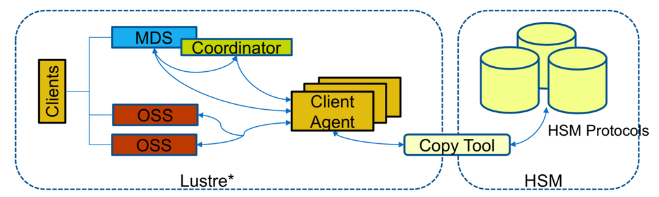
\includegraphics[width=\linewidth]{hsm架构.png}
    \caption{HSM架构}\label{fig:region-image}
\end{figure}

lustre的每个mdt都可以启动一个hsm服务,该服务又可称为Coordinator,负责收集客户端发起的hsm请求,并按照一定的策略将该请求转发到对应的Agent。 

Agent是运行在lustre客户端上的一个或者多我之前个用户进程。Agent负责接收来自Coordinator的hsm请求,并将请求解析请求,向具体的Copy tool发送HSM命令。 

Copytool则负责执行具体的hsm操作。Copytool仅响应来自于Agent的命令,其本质上是一个用户态进程。Copytool是一个针对lustre和hsm存储专用设计的数据迁移工具,例如,如果hsm后端是对象存储,提供S3接口,则Copytool需要设计成lustre的posix-to-s3的数据迁移工具。Copytool在具体执行时可以做一些其他操作,比如压缩、去重以及加密等。 

HSM架构可以设置一个集中式的策略引擎PolicyEngine。PolicyEngine是一个运行在lustre客户端的后台服务,负责实时监控lustre mdt的changelog等其他信息,之后根据用户指定的具体策略,向lustre发送HSM命令。 

\begin{figure}[!htb]
    \centering
    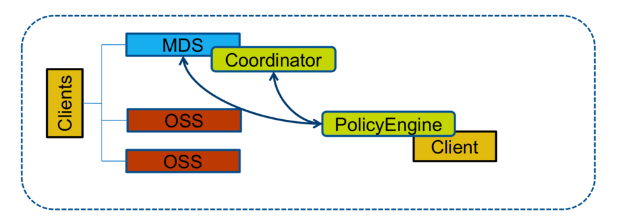
\includegraphics[width=\linewidth]{hsm.png}
    \caption{HSM PolicyEngine}\label{fig:region-image}
\end{figure}

当前针对lustre且工业上较为成熟的PolicyEngine是Robinhood





